\paragraph{K$^{0}_{S}$ Reconstruction}
\label{K0sReconstruction}

The following cuts were used to select good K$^{0}_{S}$ candidates:

\begin{enumerate}
 \item{Pion Daughter Cuts}
 \begin{enumerate}
  \item $|\eta| < 0.8$
  \item SetTPCnclsDaughters(80)
  \item SetStatusDaughters(AliESDtrack::kTPCrefic)
  \item SetMaxDcaV0Daughters(0.3)
  \item $p_{T} >$ 0.15
  \item DCA to prim vertex $>$ 0.3
 \end{enumerate}

 \item K$^{0}_{S}$ Cuts
 \begin{enumerate}
  \item $|\eta| < 0.8$
  \item $p_{T} > 0.2$
  \item $m_{PDG} -$ 13.677 MeV $< m_{inv} < m_{PDG} +$ 2.0323 MeV
  \item Cosine of pointing angle $>$ 0.9993
  \item OnFlyStatus = false
  \item Decay Length $<$ 30 cm
 \end{enumerate}  
 
\end{enumerate}

\begin{figure}
  \centering
  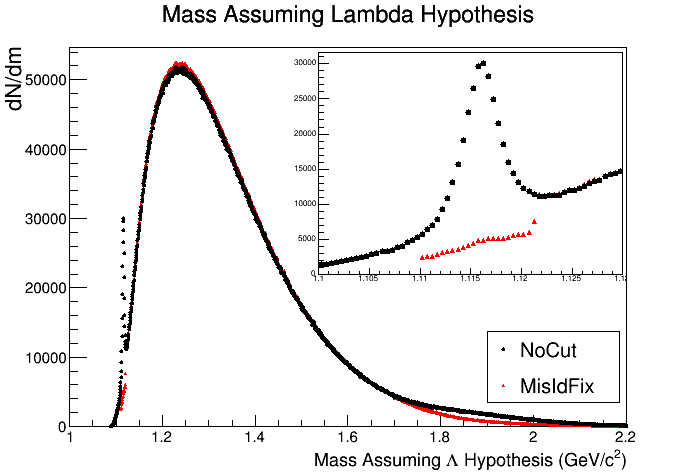
\includegraphics[width=100mm]{3_DataSelection/Figures/MassAssumingLambdaHypothesis.png}
  \caption{Here is a caption}
  \label{fig:MassAssLamHyp}
\end{figure}